\documentclass{standalone}

\usepackage{tikz}
\usepackage[T1]{fontenc}
\usepackage[tt=false, type1=true]{libertine}
\usepackage[varqu]{zi4}
\usepackage[libertine]{newtxmath}

\usetikzlibrary{shapes, positioning, calc}

\begin{document}

{\scriptsize
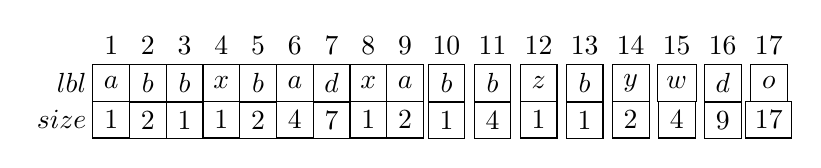
\begin{tikzpicture}
  \newcommand\arraypartspacing{0.015} % 0.03 for thick
  \newcommand\listelemminwidth{0.4675cm }
  \newcommand\listelemminheight{0.4675cm}

  \node[minimum width=\listelemminwidth, minimum height=\listelemminheight] at (0, 0) (ni1) {$1$};
  \node[draw, minimum width=\listelemminwidth, minimum height=\listelemminheight, below=-\arraypartspacing of ni1] (ni1-1) {$a$};
  \node[draw, minimum width=\listelemminwidth, minimum height=\listelemminheight, below=-\arraypartspacing of ni1-1] (ni1-2) {$1$};

  \node[left=-0.05 of ni1-1] {$lbl$};
  \node[left=-0.05 of ni1-2] {$size$};

  \foreach \label/\size [count=\prevpoid from 1, evaluate=\prevpoid as \poid using int(\prevpoid+1)] in {b/2, b/1, x/1, b/2, a/4, d/7, x/1, a/2, b/1, b/4, z/1, b/1, y/2, w/4, d/9, o/17}{
    \node[minimum width=\listelemminwidth, minimum height=\listelemminheight, right=-\arraypartspacing of ni\prevpoid] (ni\poid) {$\poid$};
    \node[draw, minimum width=\listelemminwidth, minimum height=\listelemminheight, below=-\arraypartspacing of ni\poid] (ni\poid-1) {$\label$};
    \node[draw, minimum width=\listelemminwidth, minimum height=\listelemminheight, below=-\arraypartspacing of ni\poid-1] (ni\poid-2) {$\size$};
  }
\end{tikzpicture}}

\end{document}
